\hypertarget{introduction}{%
\section{Introduction}\label{introduction1}}

To generate three-dimensional epithelial structures in vitro from planar epithelial monolayers, we chose to utilize an existing system of epithelial domes (spontaneous domes) developed by Ernest Latorre and improved by Ariadna Marin-Llaurada \cite{latorre2018,marin-llaurado2022}. This system involves seeding a Madin-Darby canine kidney (MDCK) cell monolayer on a substrate that is patterned with circular non-adhesive regions. The cells invade these regions and form a cohesive monolayer everywhere within 24 to 48 hours. Due to the active ion pumping mechanism of the MDCK cells in the apical-to-basal direction, the cells delaminate from impermeable substrates such as glass or soft PDMS gel and form spherical cap structures in the circular patterns, known as epithelial domes. Latorre and Marin-Llaurado demonstrated that they could form a variety of structures with controlled shape and size, ranging from circular to rectangular.  

This system also enables the use of 3D traction force microscopy to measure pressure. The technique involves measuring the deformation of a soft PDMS gel embedded with beads to characterize the forces and pressures applied by the cells on the substrate. This method offers an innovative approach to measuring pressure compared to the previous technique of puncturing epithelial domes with a microneedle \cite{tanner1983, choudhury2022}. It allows for the characterization of the rheology of epithelia and the discovery of interesting material properties such as the superelasticity of cells during stretching \cite{latorre2018}.  

However, the formation of epithelial domes is dependent on the ion pumping mechanism of the domes, making them spontaneous structures. Therefore, the timescales for the dome stretching are not controlled. This process can be marginally accelerated by a few hours through the use of drugs like Forskolin, which can activate transepithelial channels of NA+/K+/Cl-  \cite{klebe1995,bourke1987}. However, to build and physically control the epithelial structure, pressure control is necessary. In this chapter, we will be discussing a microfluidic chip that can inflate an epithelial monolayer into a dome while also allowing us to measure and control the forces involved.


\hypertarget{monolayer-inflator}{%
\section{Monolayer Inflator}\label{monolayer-inflator}}

Inspired by the concept of organ-on-chip microfluidic devices, we considered them to be an ideal system for controlling pressure, cell culture, and high-resolution imaging \cite{huh2010, nelson2017}. For instance, the lungs-on-chip device consists of two layers separated by a porous membrane, with one channel in the top layer for epithelia and another for endothelia. The device is assembled on a thin glass substrate, enabling high-quality imaging.  

Therefore, we conceived the idea of a MOnoLayer Inflator (MOLI) device, which utilizes a two-layer microfluidic channel with one side for epithelial monolayers and the other for the application of pressure (see fig \ref{fig_6_1}). The epithelial monolayer side is micropatterned with a protein that contains non-adhesive or less-adhesive regions for dome formation. We hypothesized that the cells would attach to the protein everywhere, even in the less adhesive regions. When pressure is applied, the cells would delaminate from the weakest point of adhesion and form a dome.  

We chose to use PDMS material for building the microfluidic chip due to its ease of use. We attempted to construct devices using plastic stickers and photopolymerizable glue, but these attempts were unsuccessful due to issues such as leakage and lack of biocompatibility \cite{sollier2011, bartolo2008}.  

\begin{figure}[h]
	\centering
	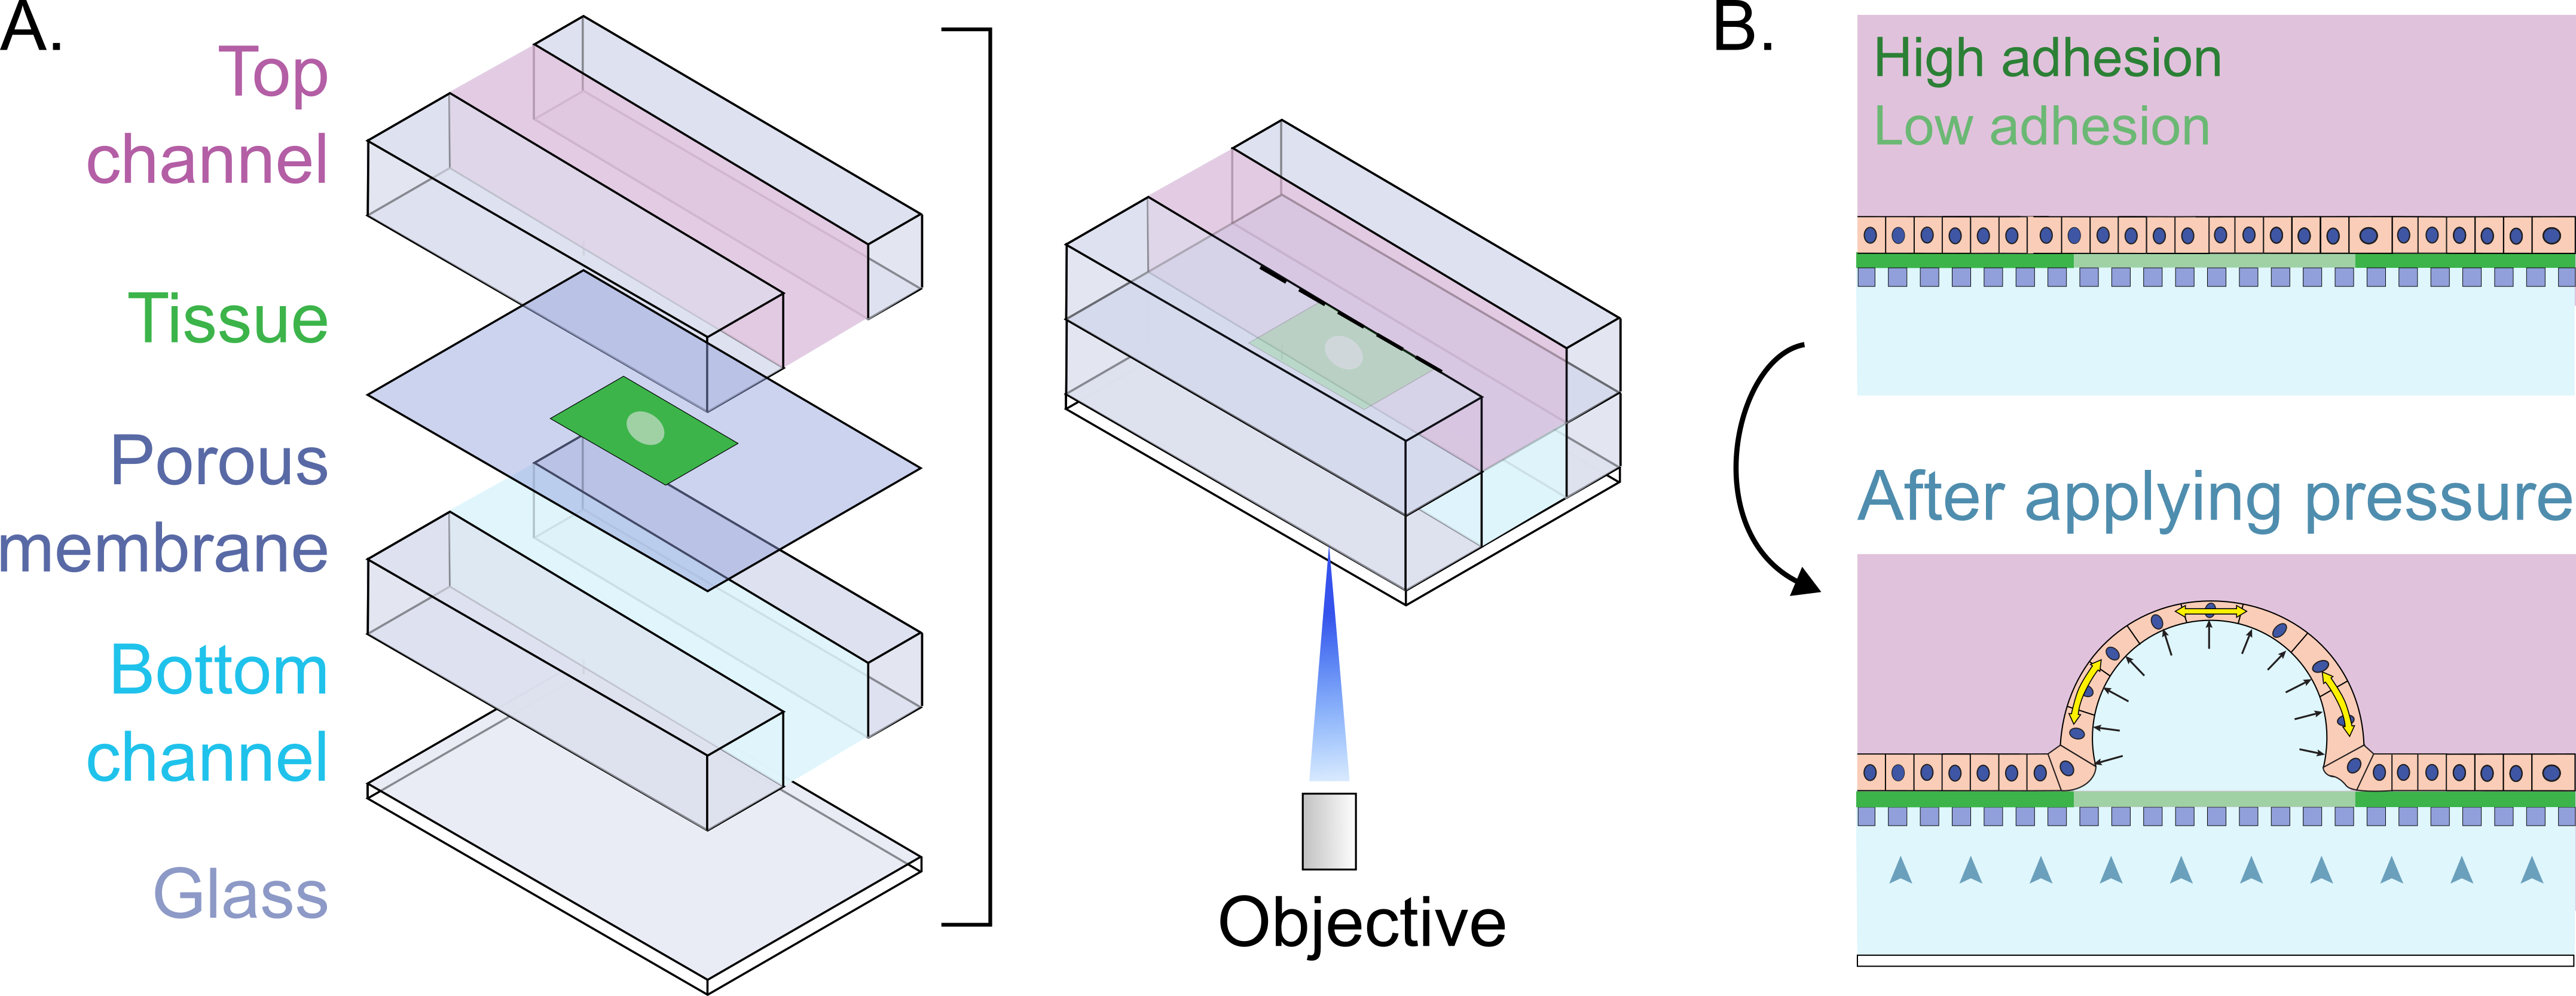
\includegraphics[width=\textwidth]{chap6_scheme.png}
	\caption{\textbf{Conceptual design of MOLI}: (A) Two layer microfluidic device with porous membrane sandwiched between. (B) Upon application of pressure, cells from low adhesion will detach to form an epithelial dome.
	}\label{fig_6_1}
\end{figure}


\hypertarget{fabrication-of-the-device}{%
\section{Fabrication of the device}\label{fabrication-of-the-device}}

The structure of the device consists of four layers: glass, bottom channel, porous membrane, and top channel. These layers are bonded together using ozone plasma activation.  

To enable high-quality imaging, the device must be mounted on a thin glass slide. Although thicker glass slides can be used, we use a glass slide \# 1.5H with a thickness of $170 \mu m$ is necessary for measuring the curvature of domes or monitoring cell stretching.  

The bottom channel must also be thin enough to ensure it is as close as possible to the working distance of most confocal microscope objectives, typically between $200\mu m$ and $1000 \mu m$. To achieve this, we fabricated the bottom layer using a thickness of $100 \mu m$. This thickness is thick enough to handle manually but not too thin to cause microfluidic problems with pressure and flow. We used a spin coating method to fabricate a thin PDMS layer and then cut the channel out of it using a desktop cutting machine (Silhouette Cameo 4, Silhouette America).  

The primary purpose of the porous membrane is to allow for pressure application while preventing cells from passing through from the cell channel to the pressure channel. We initially started with a $10\mu m$ membrane based on the literature. We attempted to use a $100 \mu m$ thin layer of PDMS with $10\mu m$ pores using photolithography, but we were unsuccessful due to producing $10\mu m$ pillars with $100 \mu m$ height, which resulted in an aspect ratio that was too high for us to get upright pillars. Therefore, we decided to use plastic (PET) membranes with $10\mu m$ pores. The thin ($10\mu m$ thick) plastic sheets were easy to handle, but we experienced bonding failures and leakages due to membrane wrinkling.  

Later, we decided to attach the PDMS thin layer to a small piece of membrane. The middle PDMS thin layer was constructed with a $1.2 mm$ hole to expose the membrane to pressure, as this dimension is approximately the size of the field of view of a 10X objective.  

The top channel was designed as a large block with a $5mm$ thickness and a $1mm$ thickness engraved channel. The thickness of the top channel was chosen arbitrarily based on the need for the block to be thick enough to plug in tubing for the application of pressure. We used a 3D printer (Solus DLP 3D Printer) to create a mold with a channel, and four inlets were added to the big block to accommodate two inlets for the bottom channel and two inlets to seed cells (see fig \ref{fig_6_1a}).

\begin{figure}
	\begin{minipage}[c]{0.6\textwidth}
		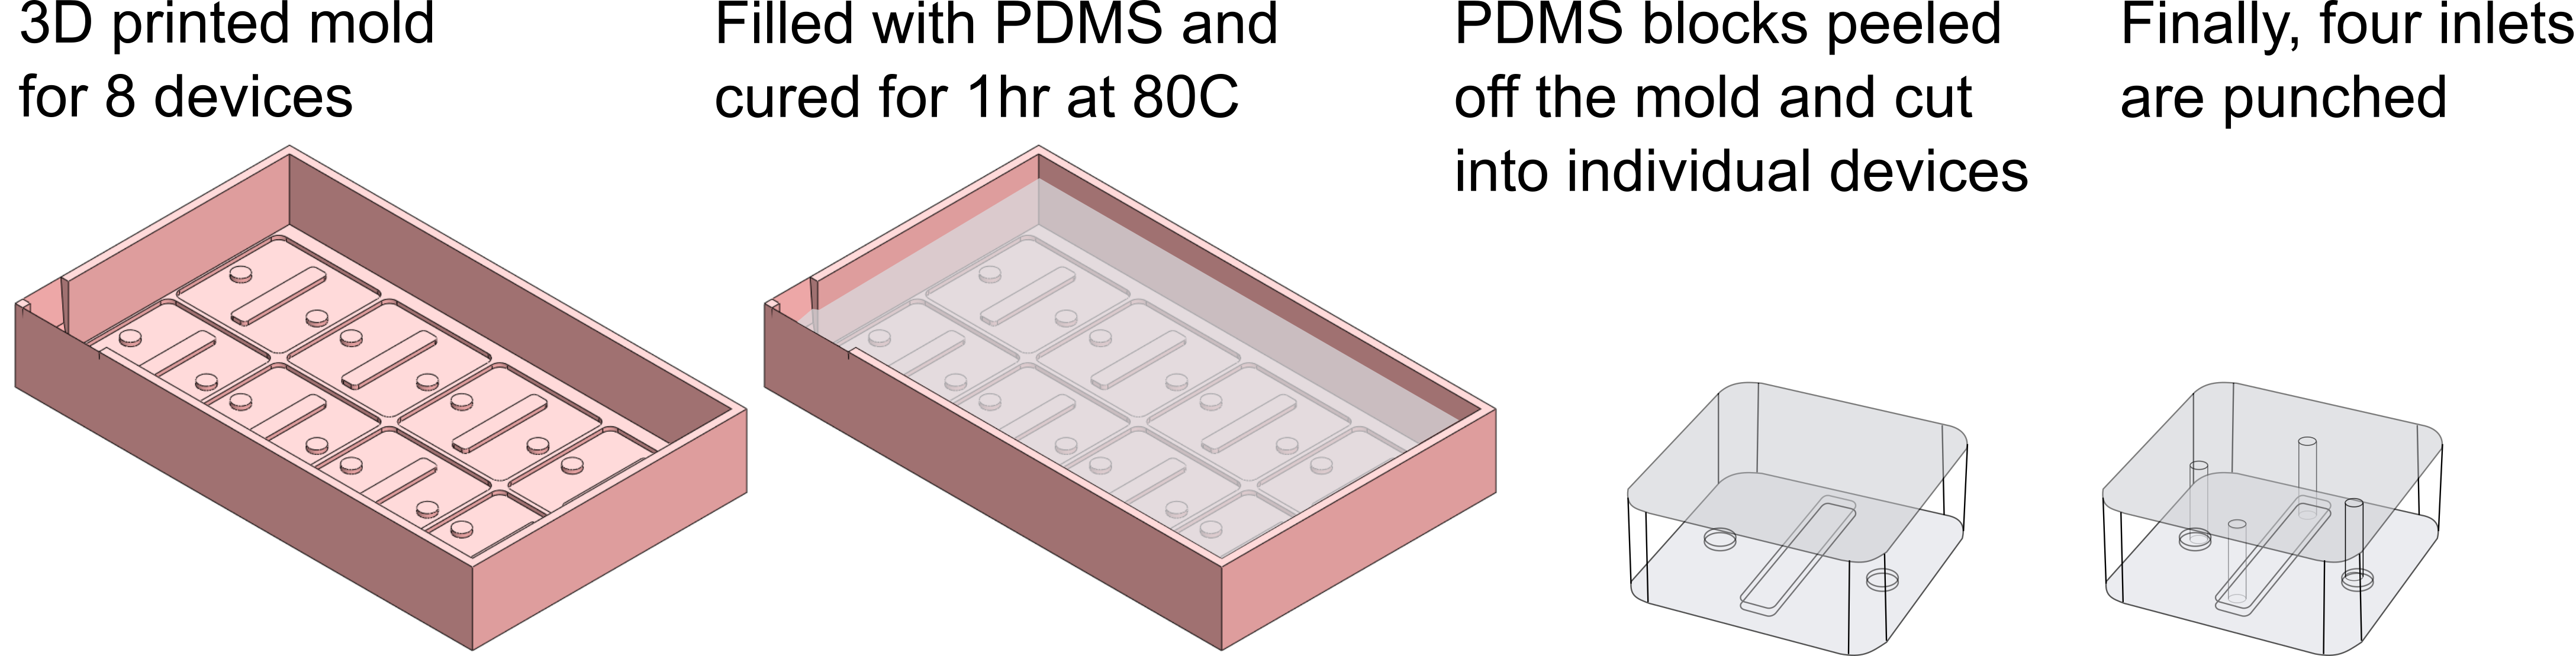
\includegraphics[width=\textwidth]{chap6_mold.png}
	\end{minipage}\hfill
	\begin{minipage}[c]{0.35\textwidth}
		\caption{\\ \textbf{3D printed mold for the device} patterned to prepare eight devices at a time. The thickness of the PDMS block is controlled with volume of PDMS poured into the mold.
		}\label{fig_6_1a}
	\end{minipage}
\end{figure}  

Finally, all the layers were bonded together in two steps using an ozone plasma cleaner (see fig \ref{fig_6_2}). First, we bonded the glass to the bottom channel and simultaneously bonded the middle layer to the top channel. Once these layers were bonded, we then bonded them to each other with the membrane sandwiched in the middle.

\begin{figure}
	\centering
	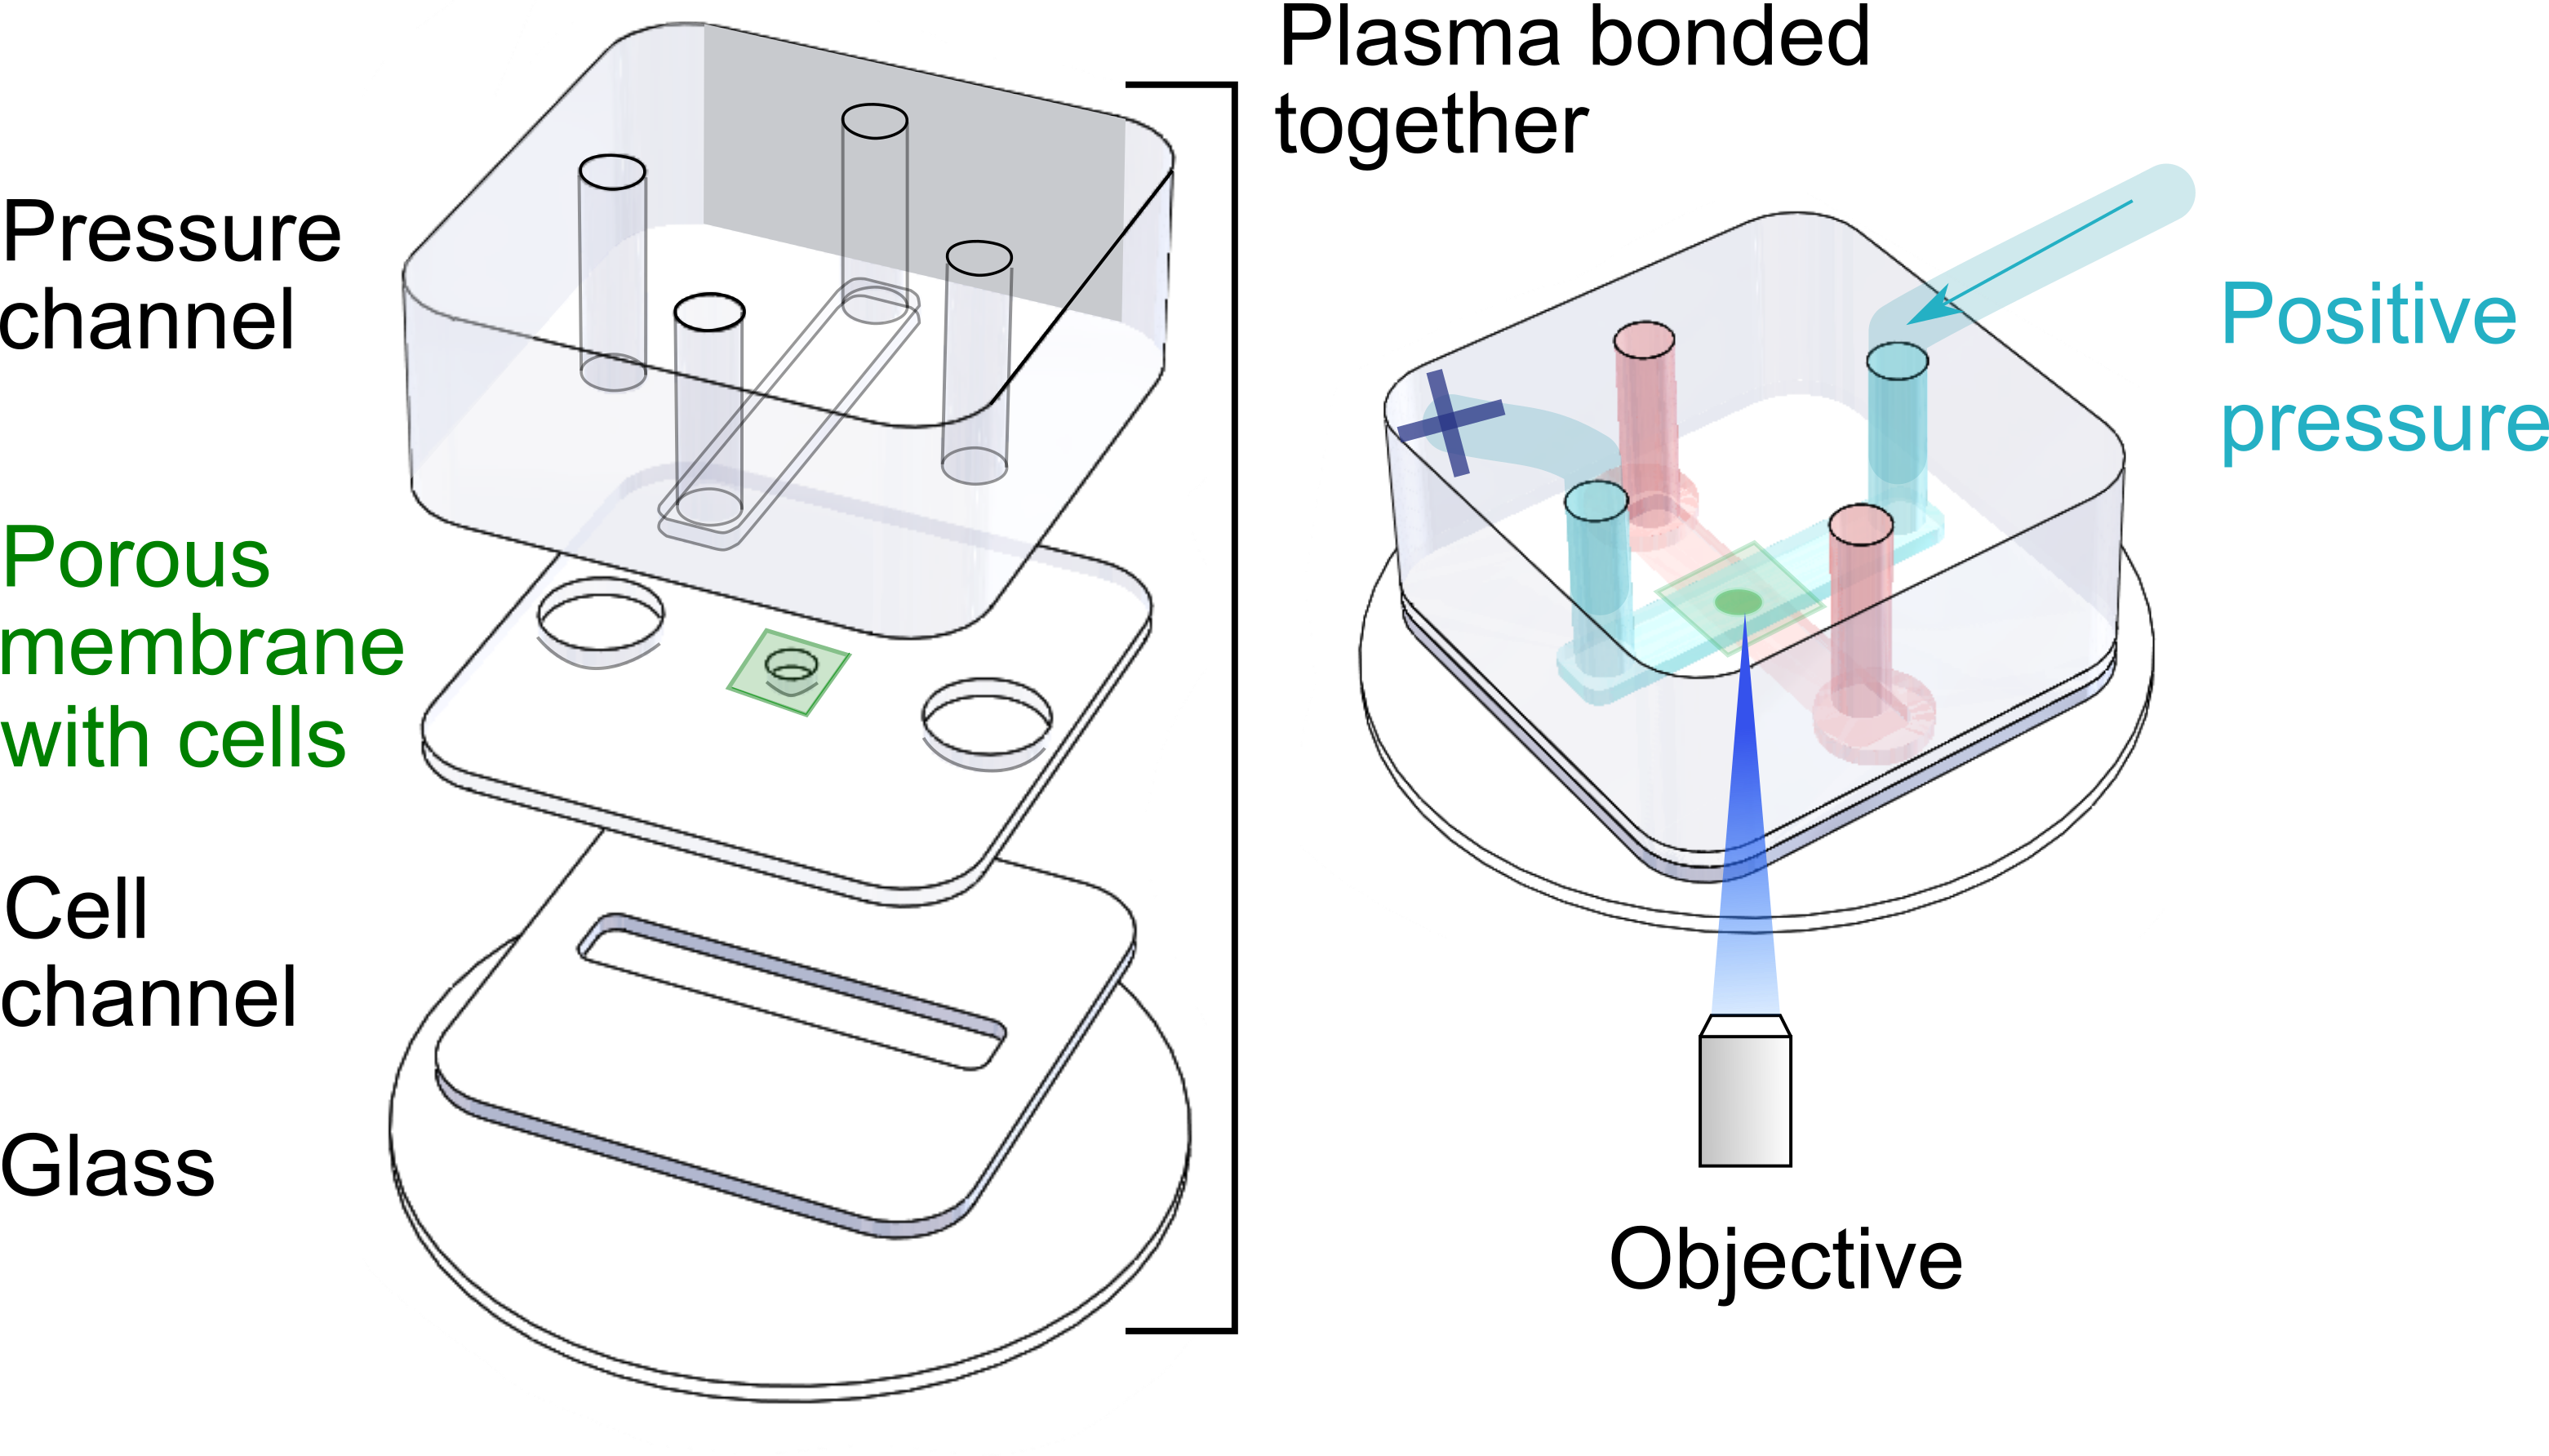
\includegraphics[width=0.75\textwidth]{chap6_realscheme.png}
	\caption{ \textbf{Fabrication of MOLI}: Four layers assembled together with ozone plasma cleaning. Each channels has a inlet and outlet. Only the pressure channel is connected to the tubing; one side connects to the reservoir and other is sealed. 
	}\label{fig_6_2}
\end{figure}

\hypertarget{protein-patterning-and-inverted-cell-culture}{%
\section{Protein patterning and "upside-down" cell
culture}\label{protein-patterning-and-inverted-cell-culture}}

After a few trials, we realized that the entire device needed to be contained in a Petri dish due to the cell culture medium. Placing the glass slide in a larger Petri dish resulted in liquid flowing underneath the glass, and any leakage during pressure application caused spillage in the microscope. Consequently, we designed the setup to fit within a glass-bottomed dish (35 mm, no. 0 coverslip thickness, Cellvis).  

In the context of the spontaneous dome system, the upper surface was accessible for various treatments and microcontact printing using a polydimethylsiloxane (PDMS) block. However, in our case, we have a completely sealed device, which necessitated the use of the photopatterning technique known as PRIMO. The PRIMO technique had been optimized previously for substrates made of glass and soft PDMS. For our setup, we had to optimize the technique for use with a plastic porous membrane, which entailed increasing laser power and protein concentration (for details see the Appendix). In brief, we first coated the surface with poly-L-lysine (PLL) and then SVA-PEG chains. Upon illumination with blue light, selective regions could be cleaved and subsequently exposed to adhesion-promoting proteins. In our experiments, we utilized fibronectin, although other proteins such as vitronectin and collagen could also be coated onto the surface.

We also had to optimize the cell seeding. Unlike in other setups where cells could be seeded in a dish, the channel required a higher concentration of cells than typical spontaneous dome experiments. We seeded $30\times 10^6$ cells/ml for one hour and then washed away the cells that did not attach within that hour.  

In our early experiments, we observed that while cells attached to the top side of the porous membrane, there were very few dome formations upon application of pressure. Additionally, the quality of imaging was poor due to imaging through the porous membrane. In the top channel, the cells were further away from the microscope objective, and we also noticed that cells were filtering through the membrane from top to bottom (see fig \ref{fig_6_4}).  

\begin{figure}[h]
	\centering
	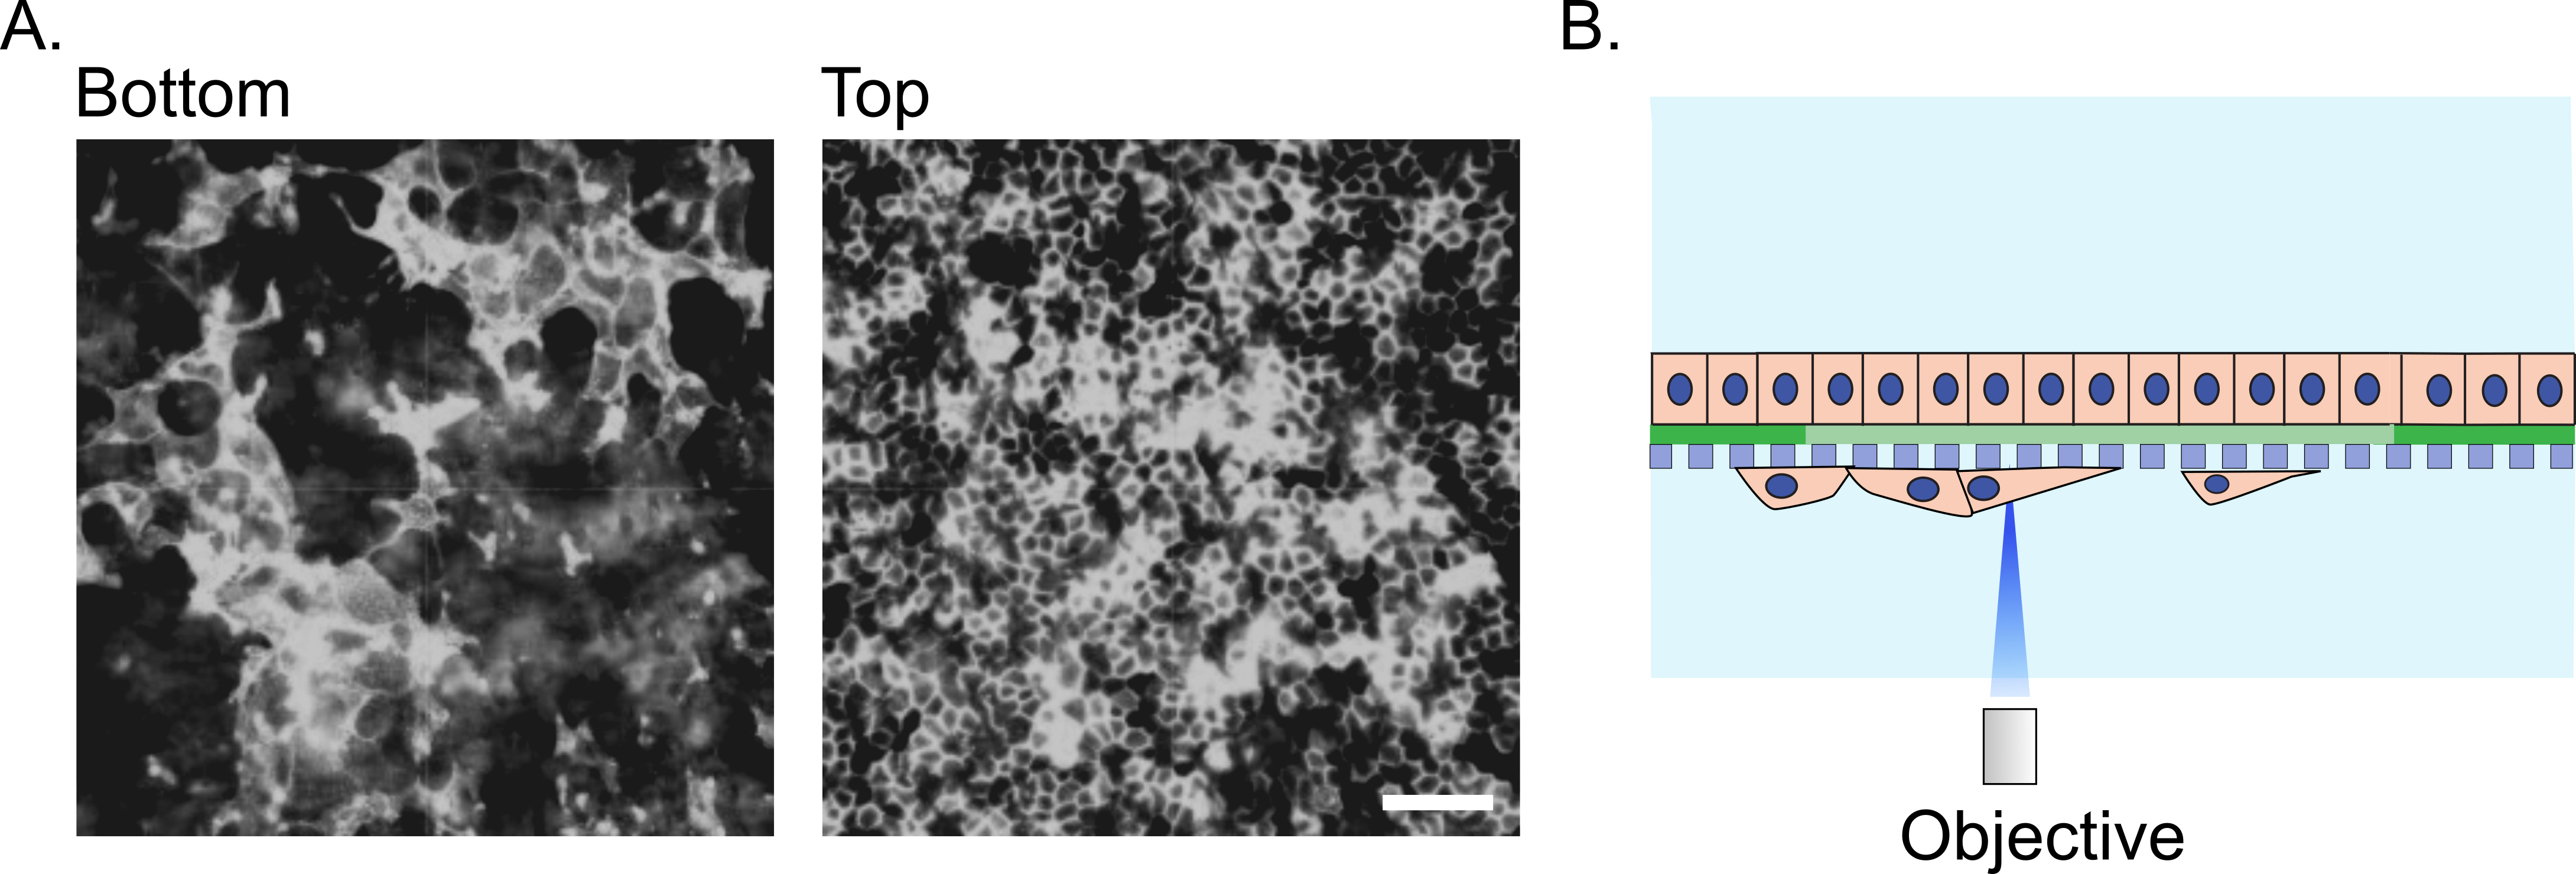
\includegraphics[width=0.75\textwidth]{chap6_cellsontop.png}
	\caption{ \textbf{Cells filtering through the membrane}: (A) Images of MDCK-CiBN CAAX GFP monolayer on the both sides of the membrane. Scale bar is $80\mu m$ (B) Schematic of imaging through the porous layer.
	}\label{fig_6_4}
\end{figure}

To prevent cells from crossing the membrane, we decided to use a membrane with smaller pore size, around $400nm$. However, imaging the green channel ($488nm$) through these pores was impossible. Therefore, we decided to change the side of seeding cells from top to bottom, which improved two things. First, imaging was better as the cells and dome were closer to the objective. Second, cells were seeded on the good side of the protein pattern.  

We termed this "upside-down" cell culture, where we would flip the device immediately upon seeding cells in the bottom channel to ensure attachment on the membrane, not the glass (see fig \ref{fig_6_5}). We had to thoroughly wash the channel to prevent cells from attaching to the glass, which would obstruct the imaging of the domes.  

Despite these improvements, the ultimate challenge was ensuring that the cell monolayer covered the non-adhesive regions. To resolve this issue, we increased the protein concentration in these regions so that cells could attach there weakly and detach first to form a dome.  


\begin{figure}[h]
	\begin{minipage}[c]{0.7\textwidth}
		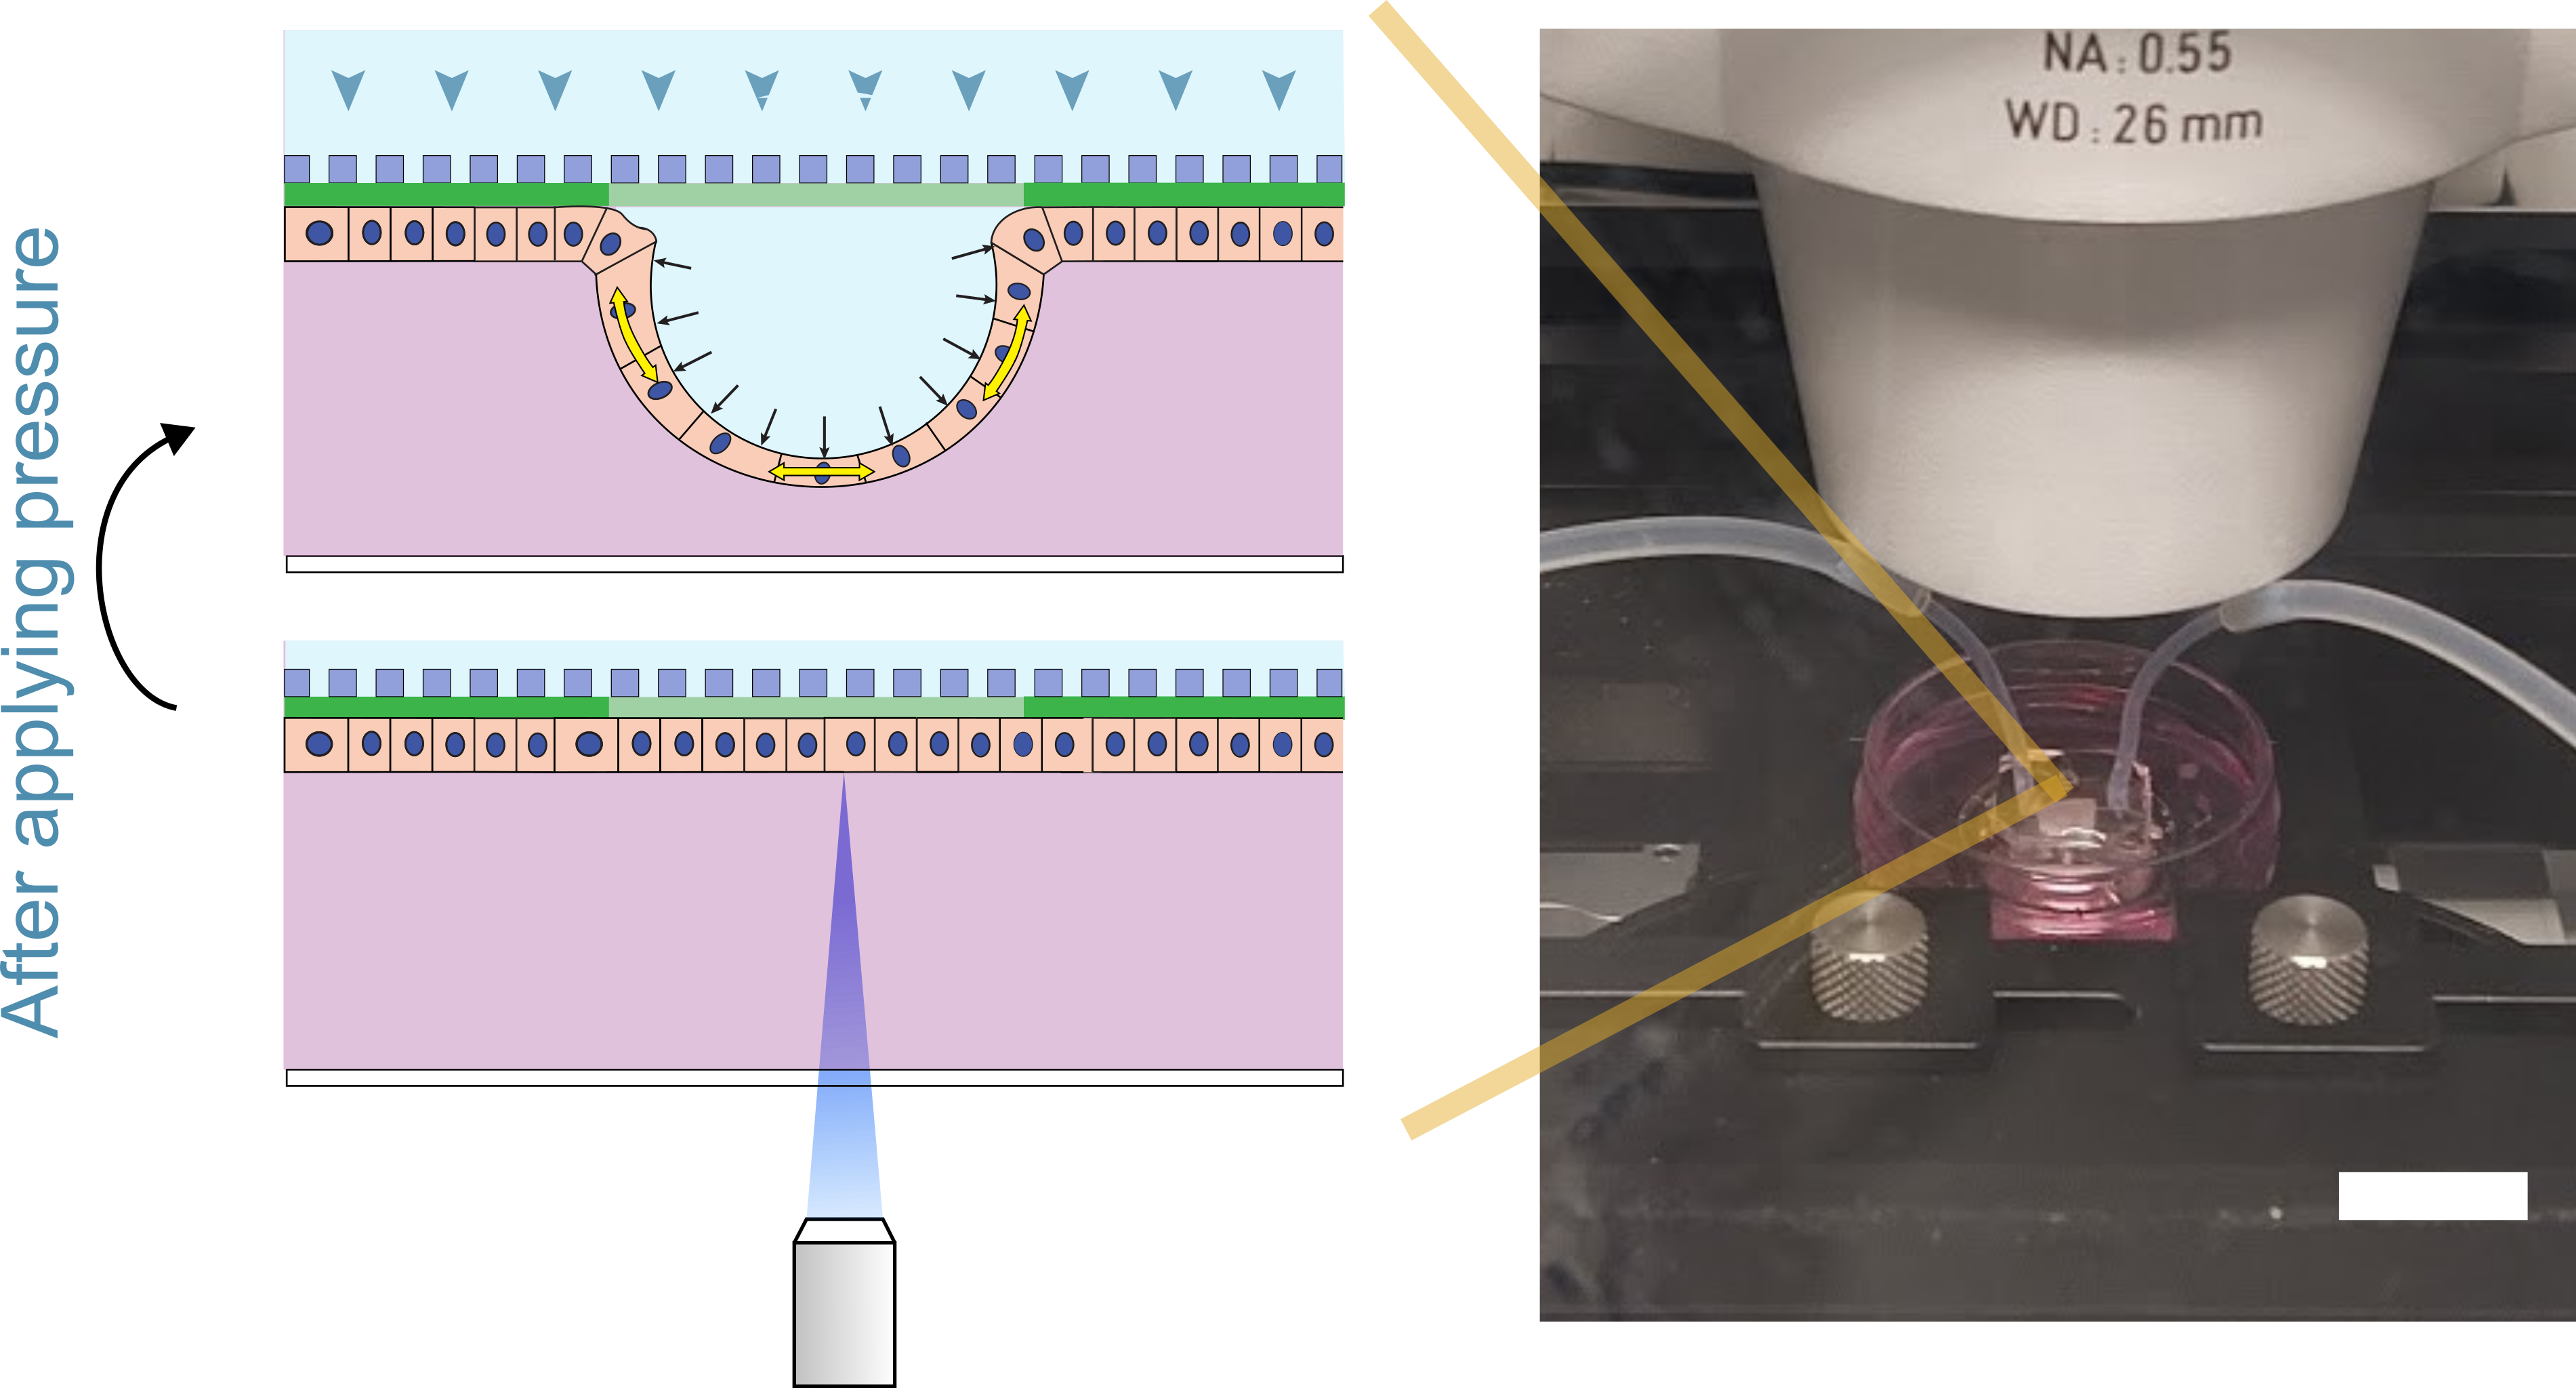
\includegraphics[width=\textwidth]{chap6_realdevice.png}
	\end{minipage}\hfill
	\begin{minipage}[c]{0.27\textwidth}
		\caption{\\ \textbf{Upside-down cell culture}: Illustration of upside-down cell culture and the experimental setup on the microscope stage.
		}\label{fig_6_5}
	\end{minipage}
\end{figure}

\hypertarget{pressure-control}{%
\section{Pressure control}\label{pressure-control}}

After optimizing protein patterning, cell culture conditions, and confocal microscopy, we turned our attention to pressure control. Our idea was to use hydrostatic pressure.  Previous studies indicated that the pressure required to form a dome is around $100Pa$, which is equivalent to $1cm$ of water column.

In early trials, we used pipette tips to apply pressure. However, we found that they were prone to bubbles and leaks. Therefore, we switched to using Polytetrafluoroethylene tubing, which was connected to a $15ml$ reservoir (falcon tube) (see fig \ref{fig_6_3}). This system allowed us to match the height of the device with the air-liquid interface in the tube, resulting in zero pressure on the monolayer. By increasing the height of the tube by $2cm$, we could apply $200Pa$ pressure to the monolayer, causing it to delaminate and form domes.  

However, we had to be careful of cavitation or bubbles getting trapped in the cell channel. To prevent this, before the experiment we had to place the media in a vacuum chamber to get rid of nascent bubbles that could grow over time. Additionally, during tubing insertion, we could introduce bubbles again. To address this issue, we used the two inlets for each channel to flush the fresh media from the reservoir, ensuring that there were no bubbles present.  

To control the pressure, we used an automatic translation stage that could be programmed to lift the reservoir. We measured the pressure by tracking the height of the stage and the zero-pressure position. With this stage, we could apply pressure in the range of $0\rightarrow 1500Pa$, and we could even apply negative pressure by setting it lower. For our experiments, we used the range of $-200\rightarrow 1300Pa$.  

\begin{figure}
	\begin{minipage}[c]{0.6\textwidth}
		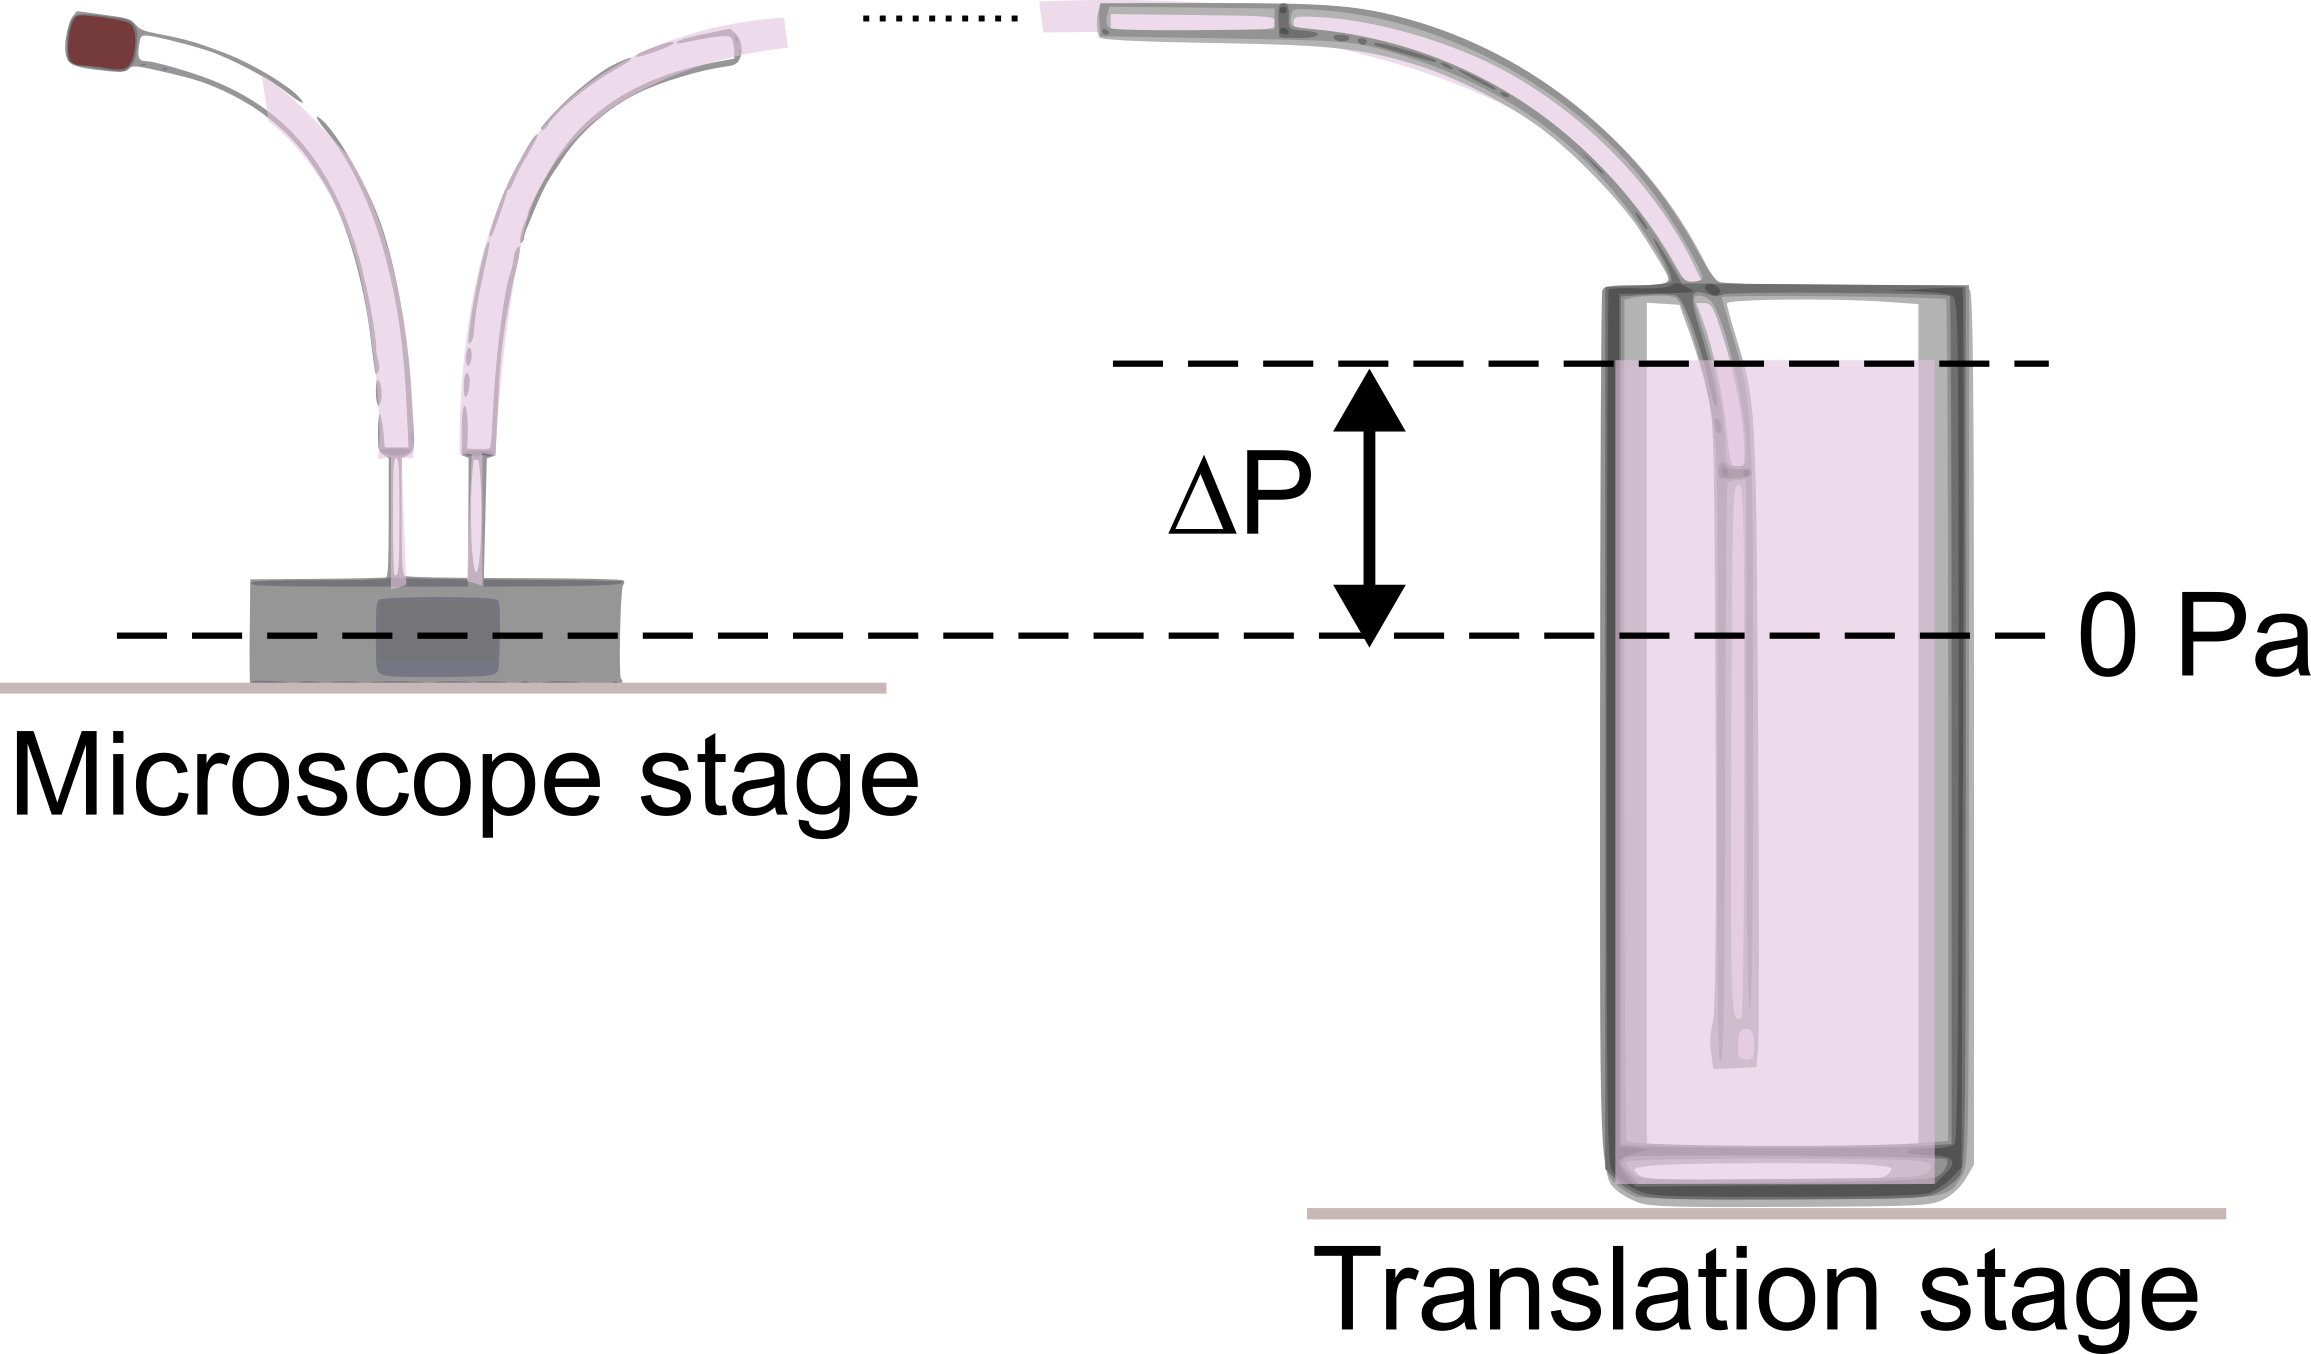
\includegraphics[width=\textwidth]{chap6_pressure.png}
	\end{minipage}\hfill
	\begin{minipage}[c]{0.35\textwidth}
		\caption{\\ \textbf{Hydrostatic pressure application}:\\ The device is positioned on a microscope stage and connected to a reservoir of media, which in turn is attached to a translation stage. By increasing the difference between the device and the air-liquid interface, we can measure and apply hydrostatic pressure.
		} \label{fig_6_3}
	\end{minipage}
\end{figure}


\hypertarget{imaging-the-epithelial-domes}{%
\section{Imaging the epithelial
domes}\label{imaging-the-epithelial-domes}}

\begin{figure}
	\begin{minipage}[c]{0.6\textwidth}
		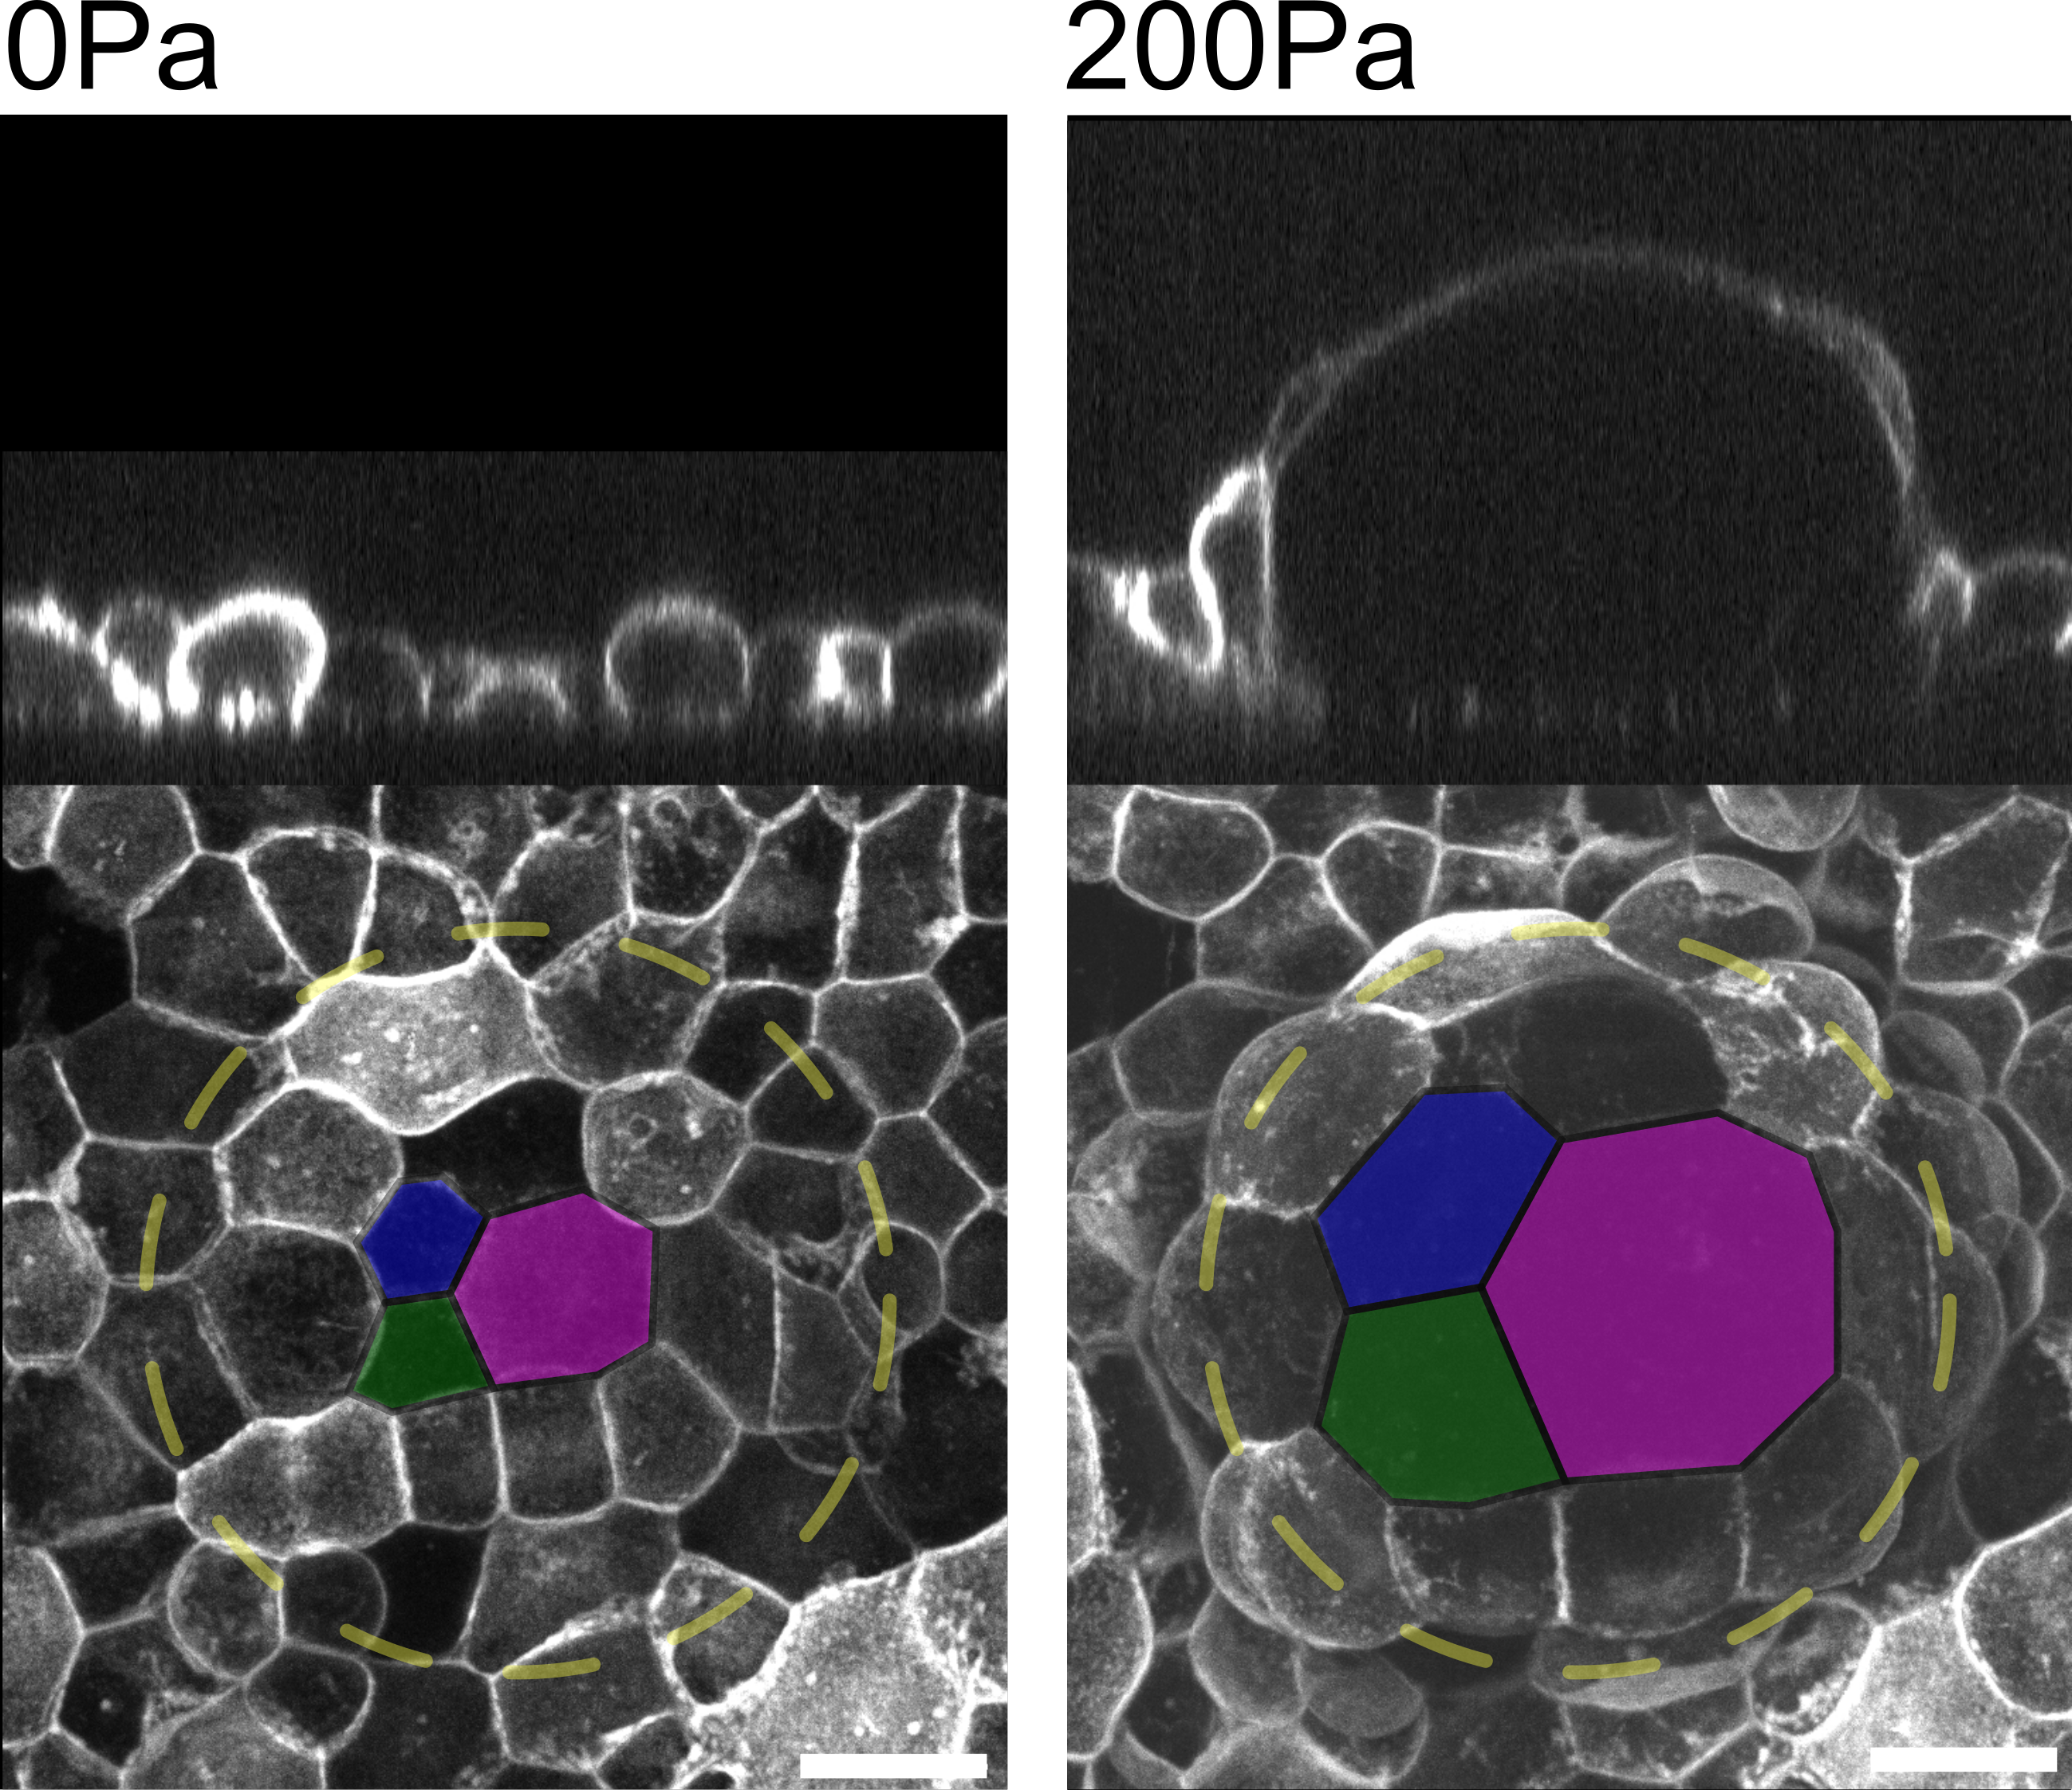
\includegraphics[width=\textwidth]{chap6_confocaldomes.png}
	\end{minipage}\hfill
	\begin{minipage}[c]{0.35\textwidth}
		\caption{\\ \textbf{Epithelial dome:}\\ Representative confocal microscopy sections of domes at 0 Pa and 200 Pa. Images in the XY plane represent the dome's maximum projection, while images in the XZ plane represent a cross section at the center plane. Three cells are highlighted with color to show the stretching during the dome inflation. Scale bar is $20 \mu m$.
		} \label{fig_6_6}
	\end{minipage}
\end{figure}

Following extensive optimization of protein patterning, cell culture conditions, and confocal microscopy techniques, we were able to generate domes in accordance with the intended pattern and exert precise control over the pressure required for their formation. To obtain images of the dome, we utilized a spinning disk confocal microscope with a 40x objective lens, which allowed us to visualize the membrane (CIBN CAAX GFP) and adhesion protein (Fibrinogen) pattern in separate channels ($488nm$ and $644nm$, respectively). By incorporating a labeled adhesion protein, we were able to track the formation of the domes with greater ease and accuracy.

Initially, we were mainly interested in spherical domes at constant pressure to characterize the epithelial mechanics (see fig \ref{fig_6_6}). We could monitor pressure, cell shape, and tissue curvature easily, enabling us to utilize Laplace's law to calculate tension. However, previous studies have tracked the dynamics of the domes at a much slower rate of $5$ minutes. In contrast, our domes could be inflated and deflated in a matter of seconds, forcing us to monitor them only by looking at the base of the dome, where the monolayer would come in and out of view.  

However, acquiring images of the dome stack using a step size of $0.5\mu m$ and height of $100 \mu m$ in a confocal microscope required three minutes, which was slower than the rate at which we could deform the dome by changing the pressure (see fig \ref{fig_6_6}). To investigate the rheology of the domes, it was necessary to monitor their dynamic response at faster pressure rates and shorter timescales, with a focus on measuring dome strain and curvature. Given the dome's inherent symmetry, imaging the mid-section of the structure provided sufficient information to characterize its material response.

With the line scanning mode of a Zeiss Airy Scan Microscope, we were able to quickly image a single line of pixels across the midsection of the dome and take a confocal z-stack along the height of the dome (see fig \ref{fig_6_7}). This provided us with a cross-section of the dome in a fraction of the time of a normal stack. By enabling piezo stage movement, we were able to image a $100\mu m$ tall dome in just $4s$, and could even track the dome height evolution through a kymograph of the central part of the dome. However, it is important to note that this form of imaging is primarily useful for tracking dome strain and curvature, and the quality of the cell images is often low. In cases where the fluorescent expression of cells on the top of the domes was inadequate, the data was much noisier.  

\begin{figure}
	\begin{minipage}[c]{0.6\textwidth}
		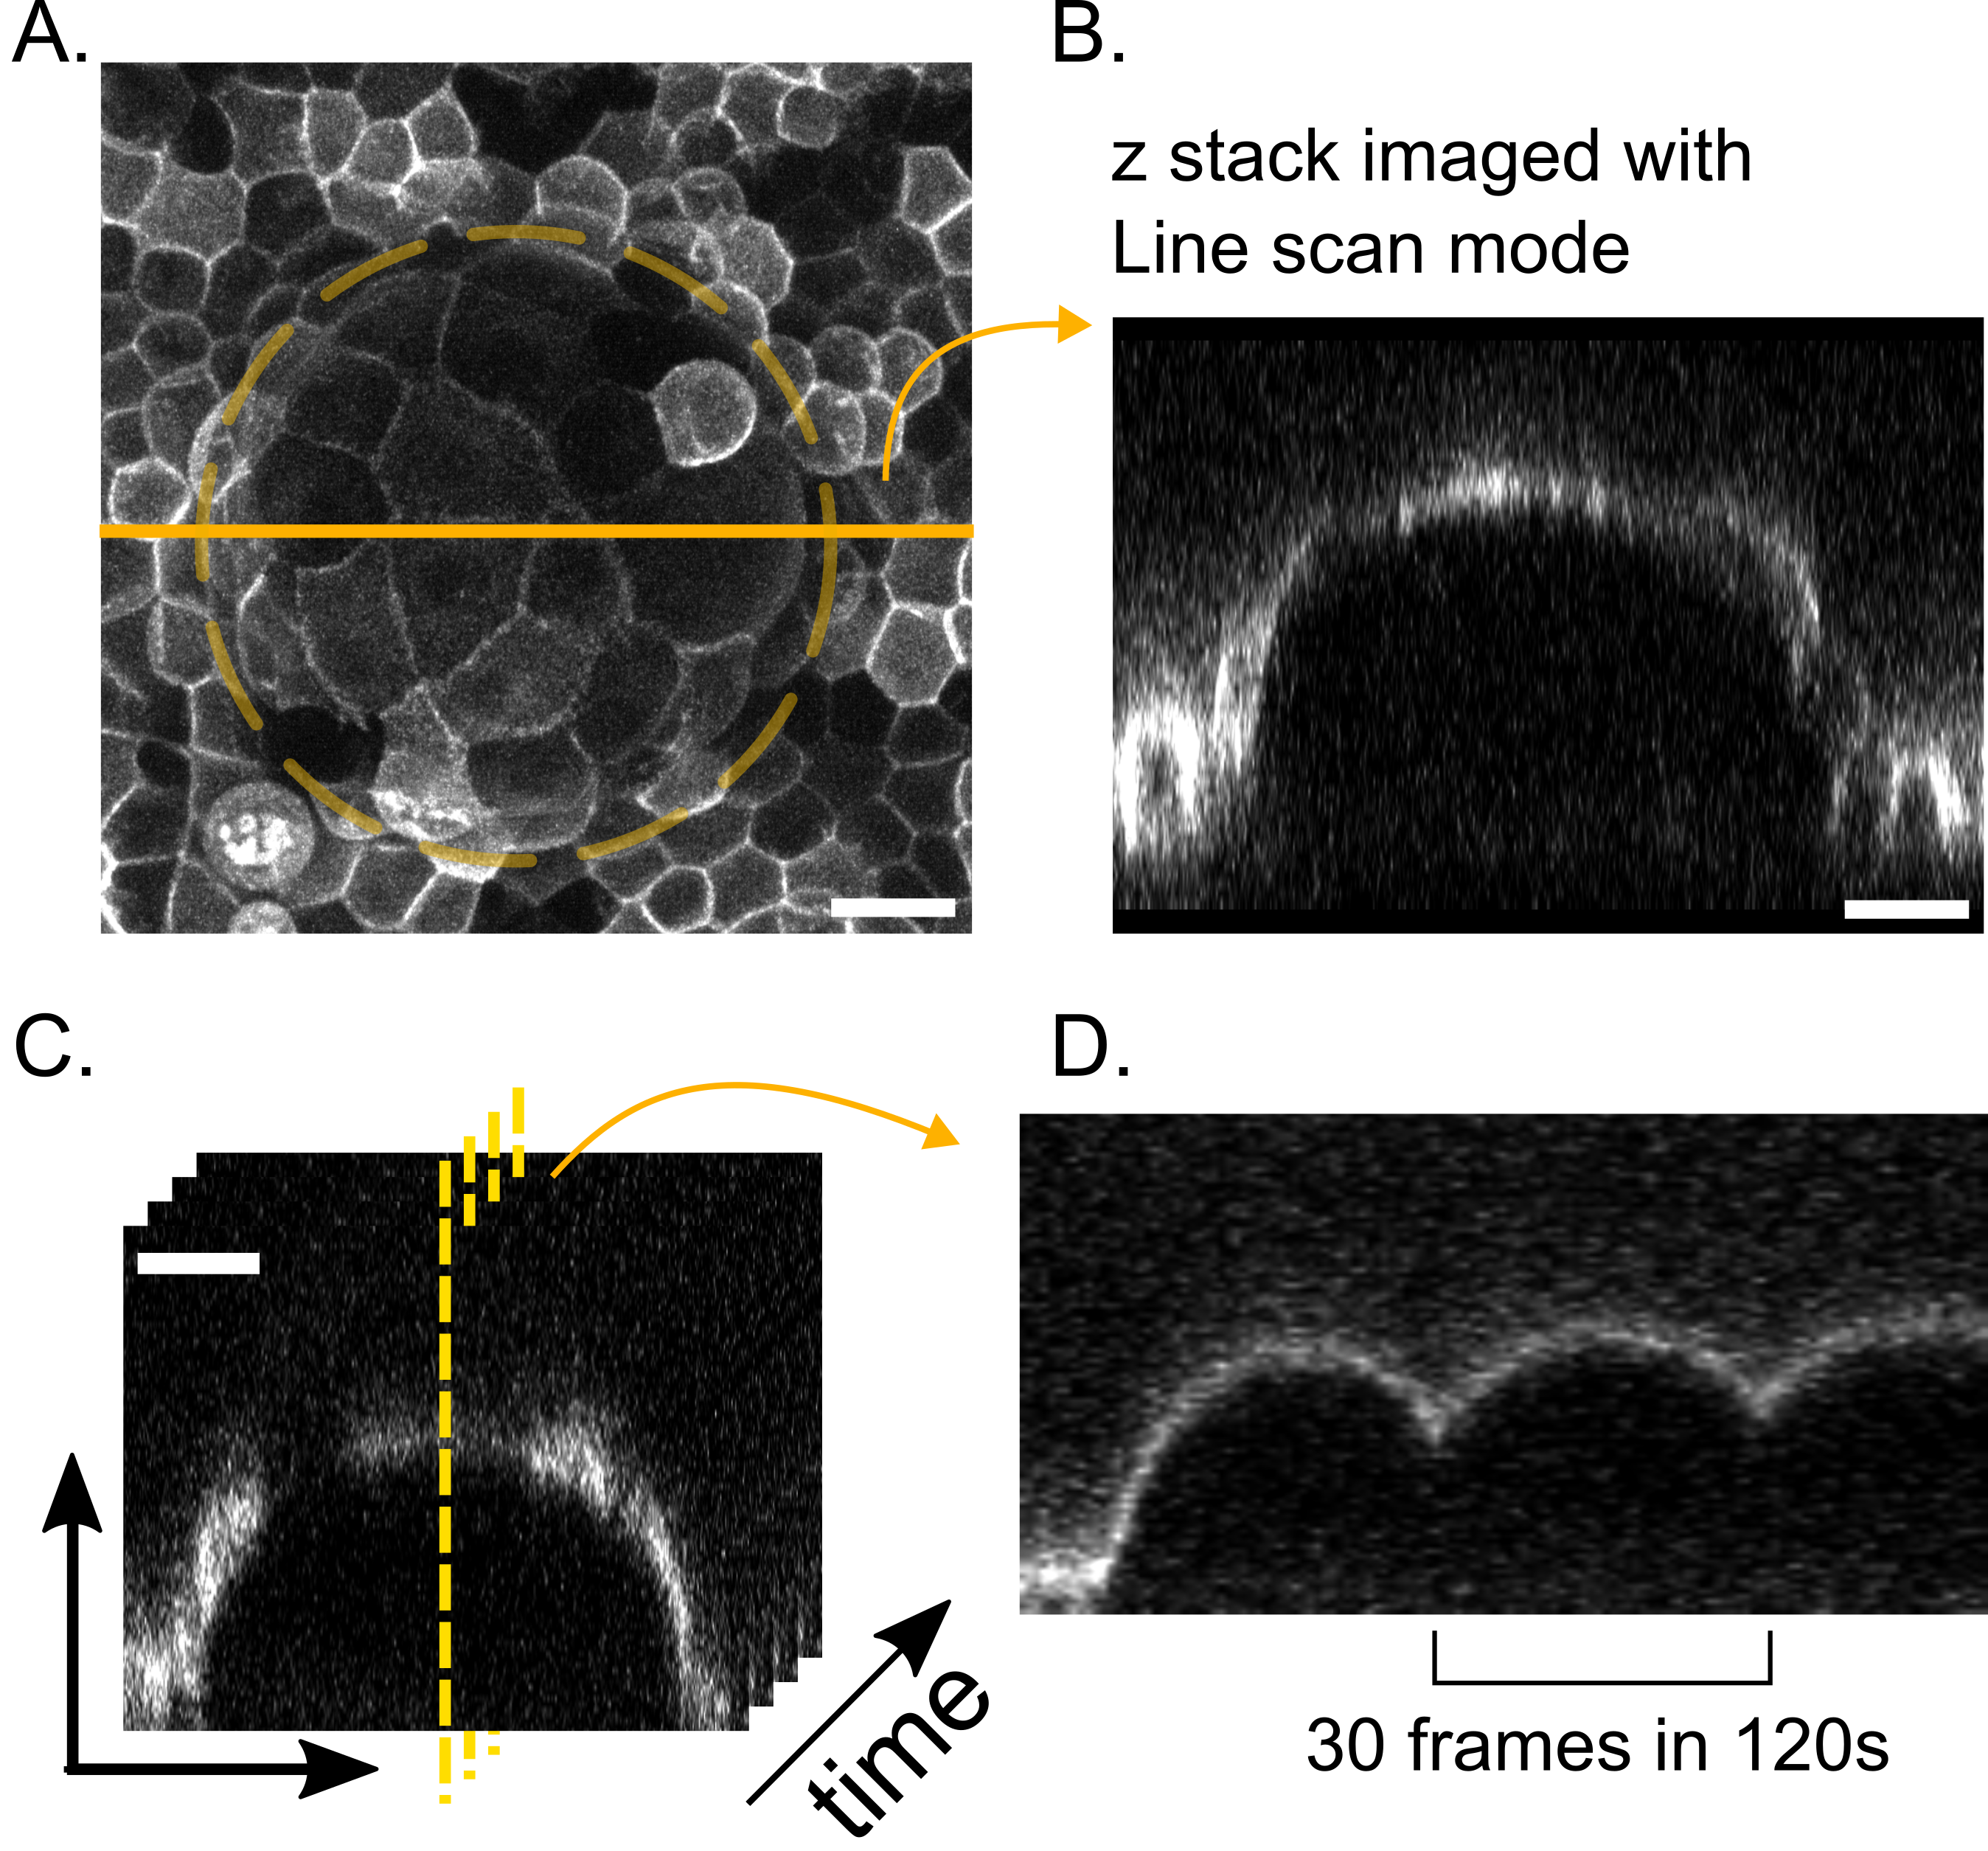
\includegraphics[width=\textwidth]{chap6_LSM.png}
	\end{minipage}\hfill
	\begin{minipage}[c]{0.35\textwidth}
		\caption{\\ \textbf{Imaging the dome with Line scanning mode:}\\ (A) Confocal microscopy image of a dome's maximum projection. (B) Midsection of the same dome imaged with the line scan mode (LSM). (C-D) Timelapse of the dome in LSM and a kymograph showing dynamics of the domes when imaged at time-step of $4s$. Scale bars are $20 \mu m$.
		} \label{fig_6_7}
	\end{minipage}
\end{figure}

\hypertarget{light-sheet-moli}{%
\section{Light-sheet MOLI}\label{light-sheet-moli}}

\begin{figure}[h]
	\centering
	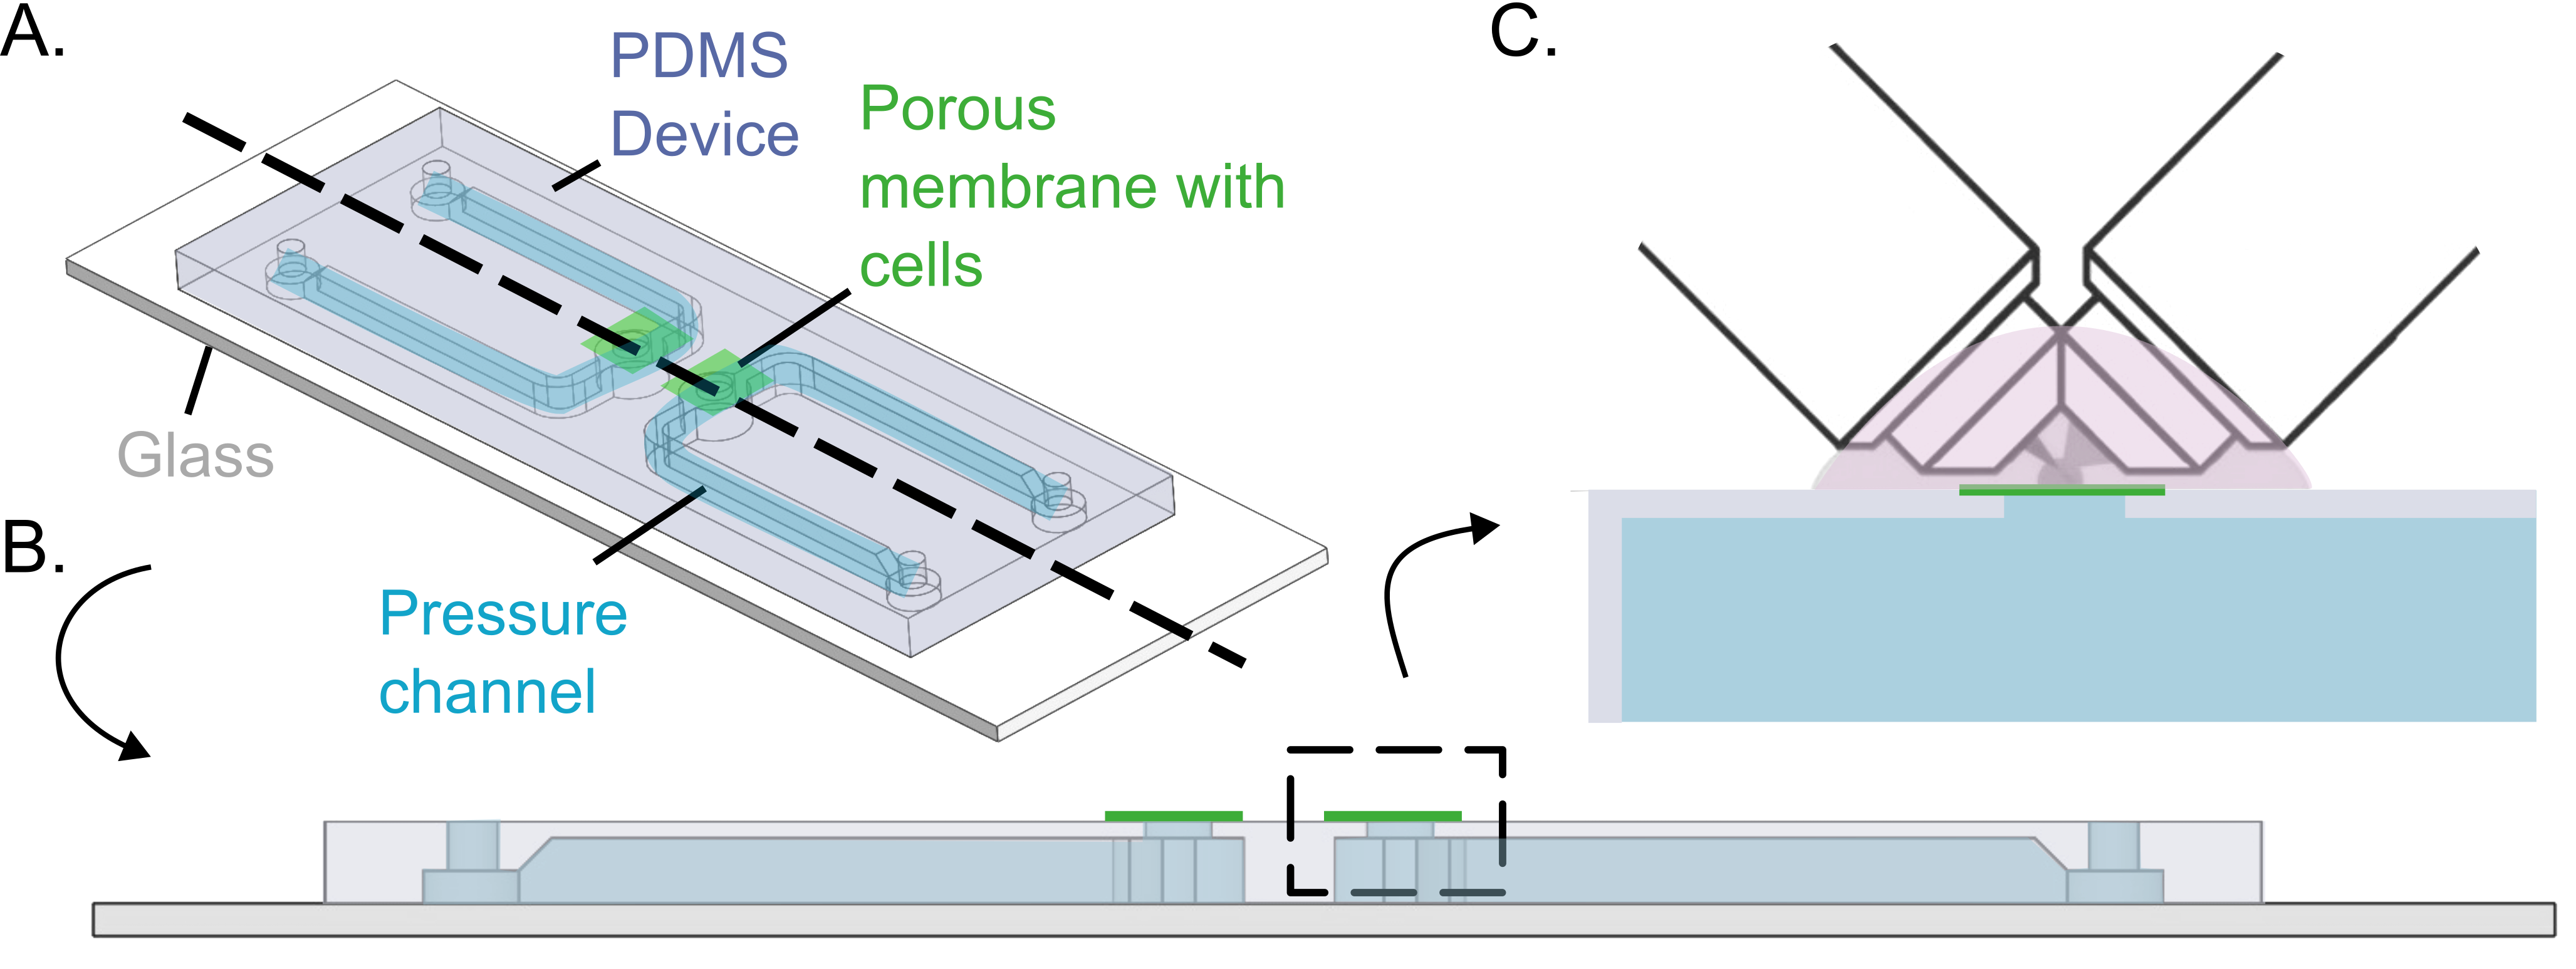
\includegraphics[width=\textwidth]{chap6_lightsheet.png}
	\caption{ \textbf{Light sheet MOLI}: (A) Isometric illustration of a single piece PDMS block engraved with two channels, so that we can have two devices in one. (B) Cross-section of the device. (C) The device is used with 40x immersion objectives coming at $45 \deg$ angle. This limits to the field of view to $332\times 332\mu m^2$.
	}\label{fig_6_8}
\end{figure}

Later in my PhD, we used a Brucker QuVi SPIM light sheet microscope to observe rapid cellular or sub-cellular changes. It has two immersion-upright 40x objectives at 45 degrees to the horizontal plane. With our expertise in fabricating devices, we designed a new setup that exposed cells and porous membranes to the top for imaging (see fig \ref{fig_6_8}).

To simplify the setup for fabrication, we inverted the normal MOLI device. This only required a pressure channel and middle layer with a hole and porous membrane. The device had to be thick enough to plug in the tubing. Since the device and channels were large, we could fabricate the mold using a Ultimaker 3D printer. We created a ridge-like protrusion so that the pressure channel and cell seeding hole could be manufactured in one go. We bonded the device to a microscope slide using unpolymerized PDMS. We were able to perform PRIMO patterning of the device by flipping it upside down. Seeding cells in this setup was easier as the cell seeding part was exposed.

As expected, we were able to apply pressure using the same system as before to generate domes. By using the imaging strategy we developed, we were able to obtain a full dome image within a mere 4 seconds, which allowed us to observe fast-moving features that were not discernible using other imaging techniques (see fig \ref{fig_6_9}).

\begin{figure}[h]
	\centering
	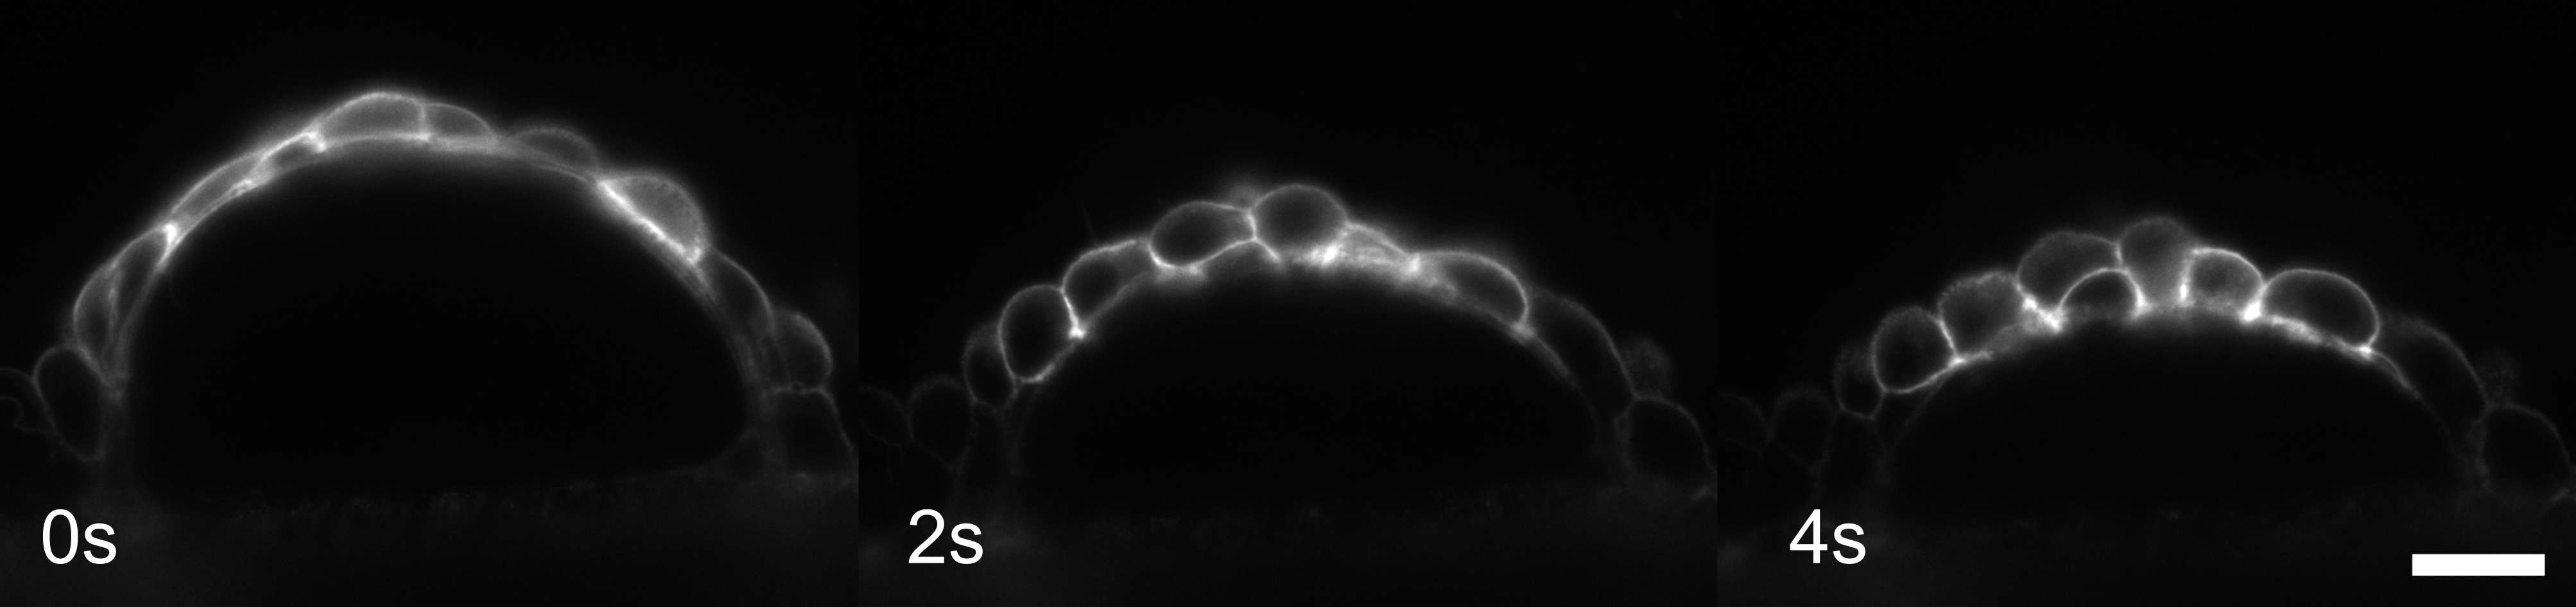
\includegraphics[width=\textwidth]{chap6_lightsheetdome.png}
	\caption{ \textbf{Dome imaged with Light sheet MOLI}: Mid-section of a dome with membrane marker imaged every $2s$. Showing the shape of individual cells undergoing changes during deflation. Scale bar is $20 \mu m$.
	}\label{fig_6_9}
\end{figure}

\newpage
\hypertarget{summary-and-discussion}{%
\section{Summary and Discussion}\label{summary-and-discussion}}

We have developed a microfluidic chip to generate 3D curved epithelia, utilizing a multilevel device consisting of two layers separated by a porous membrane. Seeding cells on the membrane in the bottom channel allowed for dome formation closer to the microscope objective, enabling high-quality confocal imaging. Hydrostatic pressure was used to control pressure under the dome dynamically, allowing for monitoring of cells and tissue behavior. Additionally, we developed imaging strategies to capture dynamics of these 3D structures faster using line scanning mode of confocal microscope or light sheet microscope.  

However, it is worth acknowledging that while the method of forming 3D epithelia described here may seem straightforward, it required many iterations of the device and other attempted methods that ultimately failed.  

We formed the domes and were able to monitor cells and tissue behavior. As shown in previous studies, the most interesting part of the system is that the complex material such as epithelial tissue to maintain mechanical equilibrium has to adopt a spherical cap shape for circular footprint. This uniform curvature and pressure implies uniform tension, for this we don't even need material properties of the tissue \cite{latorre2018,marin-llaurado2022}. The tissue tension can be measured easily by applying Laplace's law for spherical cap domes. However, in case of the non-spherical geometry, there would be anisotropic stresses which would require computational model to solve an inverse problem to go from geometry to forces \cite{marin-llaurado2022}.  

The geometry of the domes is primarily controlled by the adhesion protein pattern, but delamination can still occur. In spontaneous domes, circular footprints were found to be the most common \cite{tanner1983}, while domes formed around sharp corners can blunt themselves through delamination \cite{latorre2018}. This must be taken into consideration when creating specific geometries.  

Tissue tension and adhesion forces also interact with each other. In MDCK suspended monolayer, it is seen that cell-cell junctions are stronger than cell-substrate adhesion \cite{harris2012}, so if tension at the base of the dome exceeds the adhesion forces, it can lead to detachment and delamination.  

Moreover, unintentionally, we have created a peeling system that allows us to observe tissue being peeled off from the substrate. If the dome remains spherical, we can calculate the forces required to break cell-substrate adhesion and identify the role of molecular components of focal adhesion. However, our primary interest lies in understanding the mechanics of epithelial tissue under controlled pressure.
